% ---------------------------------------------------------------------------
% Evaluation of the v0.2 reference runtime: protocol cost, the residency
% result, and the agent-driven semantic reduction study.
% ---------------------------------------------------------------------------

\section{Protocol Cost and the Context Bound}
\label{sec:eval-ampi}

This section measures the reference runtime described in
Section~\ref{sec:algebra} rather than the earlier prototype bindings.  It
answers four questions:

\begin{enumerate}[label=Q\arabic*.]
\item What does the protocol itself cost, relative to the thing it coordinates?
\item Do the collective schedules behave as their cost models predict?
\item Does the reduce-scatter family actually deliver the residency bound that
the feasibility argument depends on?
\item With real agents evaluating a semantic operator, does the declared
algebra buy the predicted reduction in critical-path depth?
\end{enumerate}

Q1--Q3 are measured with \emph{scripted} ranks: one OS process per rank, doing
nothing but calling the protocol.  This is deliberate.  A model turn costs tens
of seconds and varies by an order of magnitude, so a measurement taken with
model-driven ranks characterises the model, not the protocol.  Q4 is measured
with Cursor subagents, one per rank, because it is a question about model
behaviour and cannot be answered any other way.  Every number below is
recomputed from the PAMPI event log in the shipped job databases; none is
reported by the code under test.

\subsection{Protocol overhead}

A ping-pong sweep between two ranks on the SQLite device fits
Equation~\ref{eq:cost}'s point-to-point terms at
$\alpha = 2.48\,\mathrm{ms}$ per step and
$\beta = 5.35\times10^{-7}\,\mathrm{s}$ per token.  Half round-trip is
2.82\,ms at 5 tokens and 2.92\,ms at 563 tokens --- flat, because at these
sizes the transaction dominates --- and rises to 22.1\,ms at 36{,}405 tokens
once the payload is spilled to the artifact store (Figure~\ref{fig:pingpong}).

The absolute numbers matter less than the ratio.  A single model turn in the
agent experiments below had a median latency of roughly 170\,s.  At
$\alpha = 2.5\,\mathrm{ms}$, one protocol step costs about
$1.5\times10^{-5}$ of one turn.  A harness can afford a great many protocol
operations per unit of agent work, which is the precondition for treating
coordination as something to be specified explicitly rather than minimised.

The sweep also exercises the receiver-driven rendezvous switch.  At 4{,}545
tokens the transfer degrades from eager to rendezvous and the receiver is
charged 27 tokens --- the structural digest --- instead of the payload, a
$168\times$ reduction; at 36{,}405 tokens the same 27-token digest is a
$1348\times$ reduction.  The body remains addressable and is fetched only if
the receiver decides to pay for it.

\begin{figure}[t]
\centering
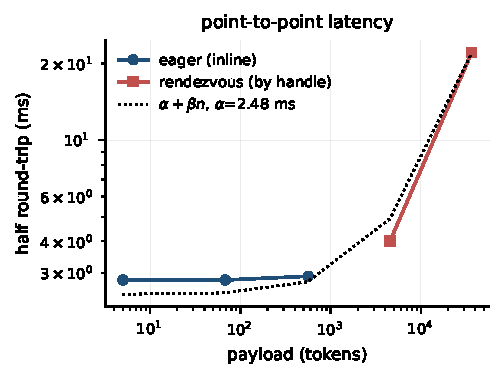
\includegraphics[width=\columnwidth]{figures/pingpong.pdf}
\caption{Point-to-point half round-trip against payload size. Latency is flat
while messages are delivered inline and rises once the receiver-driven switch
sends them by reference instead; the dotted line is the fitted
$\alpha + \beta n$ model.}
\label{fig:pingpong}
\end{figure}

\subsection{Collective schedules}

Figure~\ref{fig:collectives} shows barrier and allreduce latency against
communicator size for every implemented schedule.  Two observations, one
expected and one not.

The expected one: step counts follow the analysis exactly.  At $p=32$ the
dissemination barrier executes 10 steps against the linear barrier's 62, and
the binomial allreduce 15 against the ring's 281.

The unexpected one: fewer steps does not always mean less time on this device.
The dissemination barrier is \emph{slower} than the linear barrier at every
$p \ge 4$ --- 269\,ms against 178\,ms at $p=32$ --- despite using a sixth of
the steps.  The reason is that $\alpha$ is not uniform.  A dissemination round
is a strict alternation of send and blocking receive, so each of its 10 steps
pays a full polling round-trip, while the linear barrier's root issues 31
receives that are already satisfied by the time it asks.  The Hockney model
assumes a single $\alpha$ for every step; on a store-based transport the
effective $\alpha$ depends on whether a step waits.  We report this because it
is exactly the kind of thing a decision function has to be tuned for, and
exactly the reason MPI implementations ship measured decision files rather than
deriving the choice from step counts.

\begin{figure}[t]
\centering

\includegraphics[width=\columnwidth]{figures/collectives.pdf}
\caption{Collective latency against communicator size, scripted ranks, SQLite
device. Step counts follow the analysis, but the dissemination barrier's
fewer, strictly-serialised steps lose to the linear barrier's pipelined ones.}
\label{fig:collectives}
\end{figure}

\subsection{Peak context residency}
\label{sec:eval-residency}

Figure~\ref{fig:residency} reports the quantity the feasibility argument turns
on: the largest number of tokens a rank must hold simultaneously, measured
directly from the collective step machine rather than inferred.  Each rank
contributes 256 keyed entries, so the reduced vector grows with $p$ --- a weak
scaling sweep, which is the regime a harness is actually in when it adds
agents to cover more material.

The separation is unambiguous and matches Table~\ref{tab:allreduce-cost}.
Recursive doubling and the binomial tree hold $1.50n$ tokens at every $p$
tested, from $p=4$ to $p=32$.  Recursive-halving reduce-scatter falls from
$0.68n$ at $p=4$ to $0.09n$ at $p=32$.  In absolute terms the reduce-scatter
residency is essentially \emph{constant} --- 10.8\,k, 10.7\,k, 11.0\,k and
11.7\,k tokens at $p = 4, 8, 16, 32$ --- because $n/p$ is held fixed by the
weak-scaling design, while the doubling family's residency grows with the
vector to 197\,k tokens at $p=32$.

That last figure is the point.  At $p=32$ the reduced vector is 127{,}776
tokens.  Under a 128\,k-token context window, an allreduce that materialises
the vector at every rank cannot run: it needs 197\,k tokens resident, more than
the window, and no amount of patience fixes it.  Reduce-scatter completes the
same reduction with 9\% of the vector resident.  The decision function reaches
this conclusion in closed form before any message is sent, and reports it:
\code{ampi plan} marks recursive doubling inadmissible with the reason
``peak residency of 197033 tokens exceeds the rank context limit''.

\begin{figure*}[t]
\centering
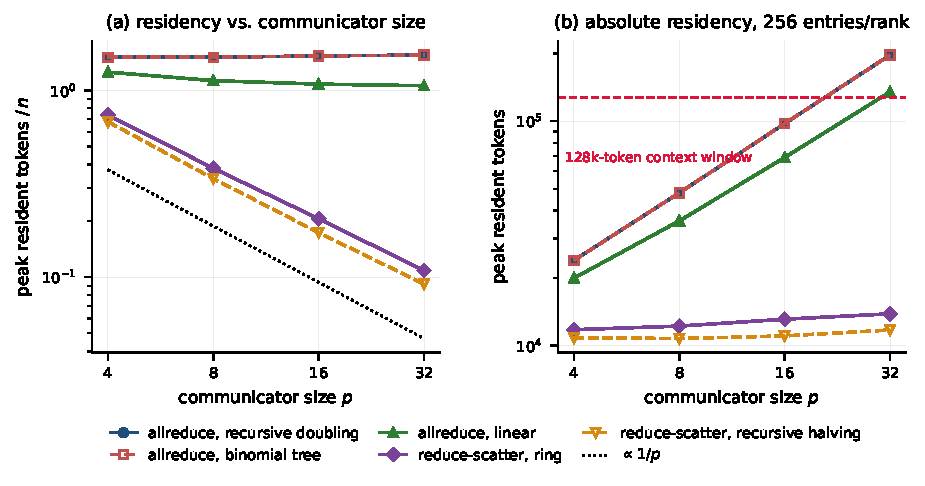
\includegraphics[width=\textwidth]{figures/residency.pdf}
\caption{Peak resident tokens per rank during an allreduce of a keyed vector,
measured from the step machine, weak scaling at 256 entries per rank. Left:
residency relative to the vector size $n$. Right: absolute residency against a
128\,k-token context window; above the dashed line the operation cannot be
performed at all. The reduce-scatter family is the only one whose reduction
phase residency falls with $p$.}
\label{fig:residency}
\end{figure*}

\subsection{One-sided operations under contention}

Uncontended window operations are cheap and flat: put 0.09\,ms, get 0.04\,ms,
atomic fetch-and-add 0.08\,ms, lease acquisition 0.09--0.12\,ms, across $p=2$
to $p=32$.  What grows is contention.  With every rank performing a
read-modify-write on one shared cell, failed compare-and-swaps rise from 0 at
$p=2$ to 2, 4, 19 and 100 at $p=4, 8, 16, 32$ (Figure~\ref{fig:contention}) ---
superlinear, as the Universal Scalability Law's coherency term
predicts~\cite{gunther2007usl}.

For a byte-oriented store those retries are nearly free.  For an agent they are
not: a lost compare-and-swap on an artifact means the agent must re-read, re-apply
its edit, and in the semantic case re-think it, at model cost.  This is the
quantitative case for the window API offering \code{win-claim} and leases
rather than only put and get: a work item claimed by compare-and-swap is
claimed once, whereas a work item taken by convention is taken by however many
agents happen to look at the same moment.

\begin{figure}[t]
\centering
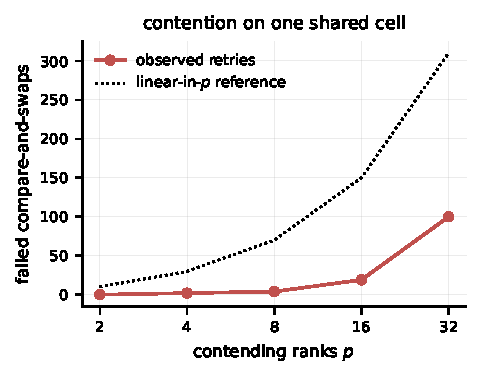
\includegraphics[width=\columnwidth]{figures/contention.pdf}
\caption{Failed compare-and-swaps on a single shared window cell as the number
of contending ranks grows. Retries are cheap for bytes and expensive for
agents, which is why the protocol offers atomic claim rather than leaving
mutual exclusion to convention.}
\label{fig:contention}
\end{figure}

\subsection{Two transports behind one interface}

An abstract device interface with one implementation behind it is an
indirection, not an interface.  The reference runtime therefore ships two
devices: the SQLite device, in which every rank opens one durable file and a
single writer serialises everything, and a filesystem device with no
coordinator on the data path, in which a message is a file written to a
temporary name and \code{rename(2)}-d into the destination rank's mailbox, and
a claim is a second rename that only one racing claimant can win.  They bracket
the design space real MPI implementations occupy: one behaves like a shared or
offloaded fabric where a single agent observes all traffic, the other like a
distributed-memory fabric where nobody does.

Both pass the same device conformance suite, which tests the four concurrency
properties the layers above depend on rather than functionality: that
\code{match} hands a record to exactly one claimant under eight concurrent
claimants, that \code{cas} rejects a stale version and admits exactly one of
six racing writers, that leases exclude and expire, and that the ticket counter
never repeats across 150 concurrent increments.

Writing that suite found a real defect in the SQLite device.  Its \code{match}
originally issued the select and the claiming update as two autocommit
statements; under contention two ranks could both read the same posted message
before either wrote, and 40 work items were handed out 181 times.  This is
precisely the duplicated-work failure that multi-agent harnesses report, in the
one component whose entire job is to prevent it, and it was invisible until the
suite ran eight claimants against it concurrently.  We mention it because the
lesson generalises: the coordination guarantees an agent protocol advertises
are exactly the ones that will be quietly wrong unless something tests them
under real concurrency.
